\subsection{Multiplicación de Matrices Cuadradas}

\subsubsection{Tiempo de Ejecución}

En el análisis de los resultados experimentales, se observa que
el algoritmo de Strassen supera al algoritmo de Naive en tiempo de
ejecución para matrices densas, en la escala logarítmica 
($10^{-2}$ a $10^3$ ms), Strassen muestra tiempos superiores a Naive 
en la gran mayoría de las dimensiones evaluadas (de $n = 64$ a $n = 1024$). 
Solo en $n = 16$ se aprecia un tiempo ligeramente menor.

\vspace{0.4cm}

Ademas, se observa que el tiempo de ejecución de Strassen crece
a un ritmo más lento que el de Naive, lo que indica que la
complejidad asintótica de Strassen es menor, como se aprecia 
en la Figura~\ref{fig:matrix_time}:

\begin{figure}[H]
    \centering
    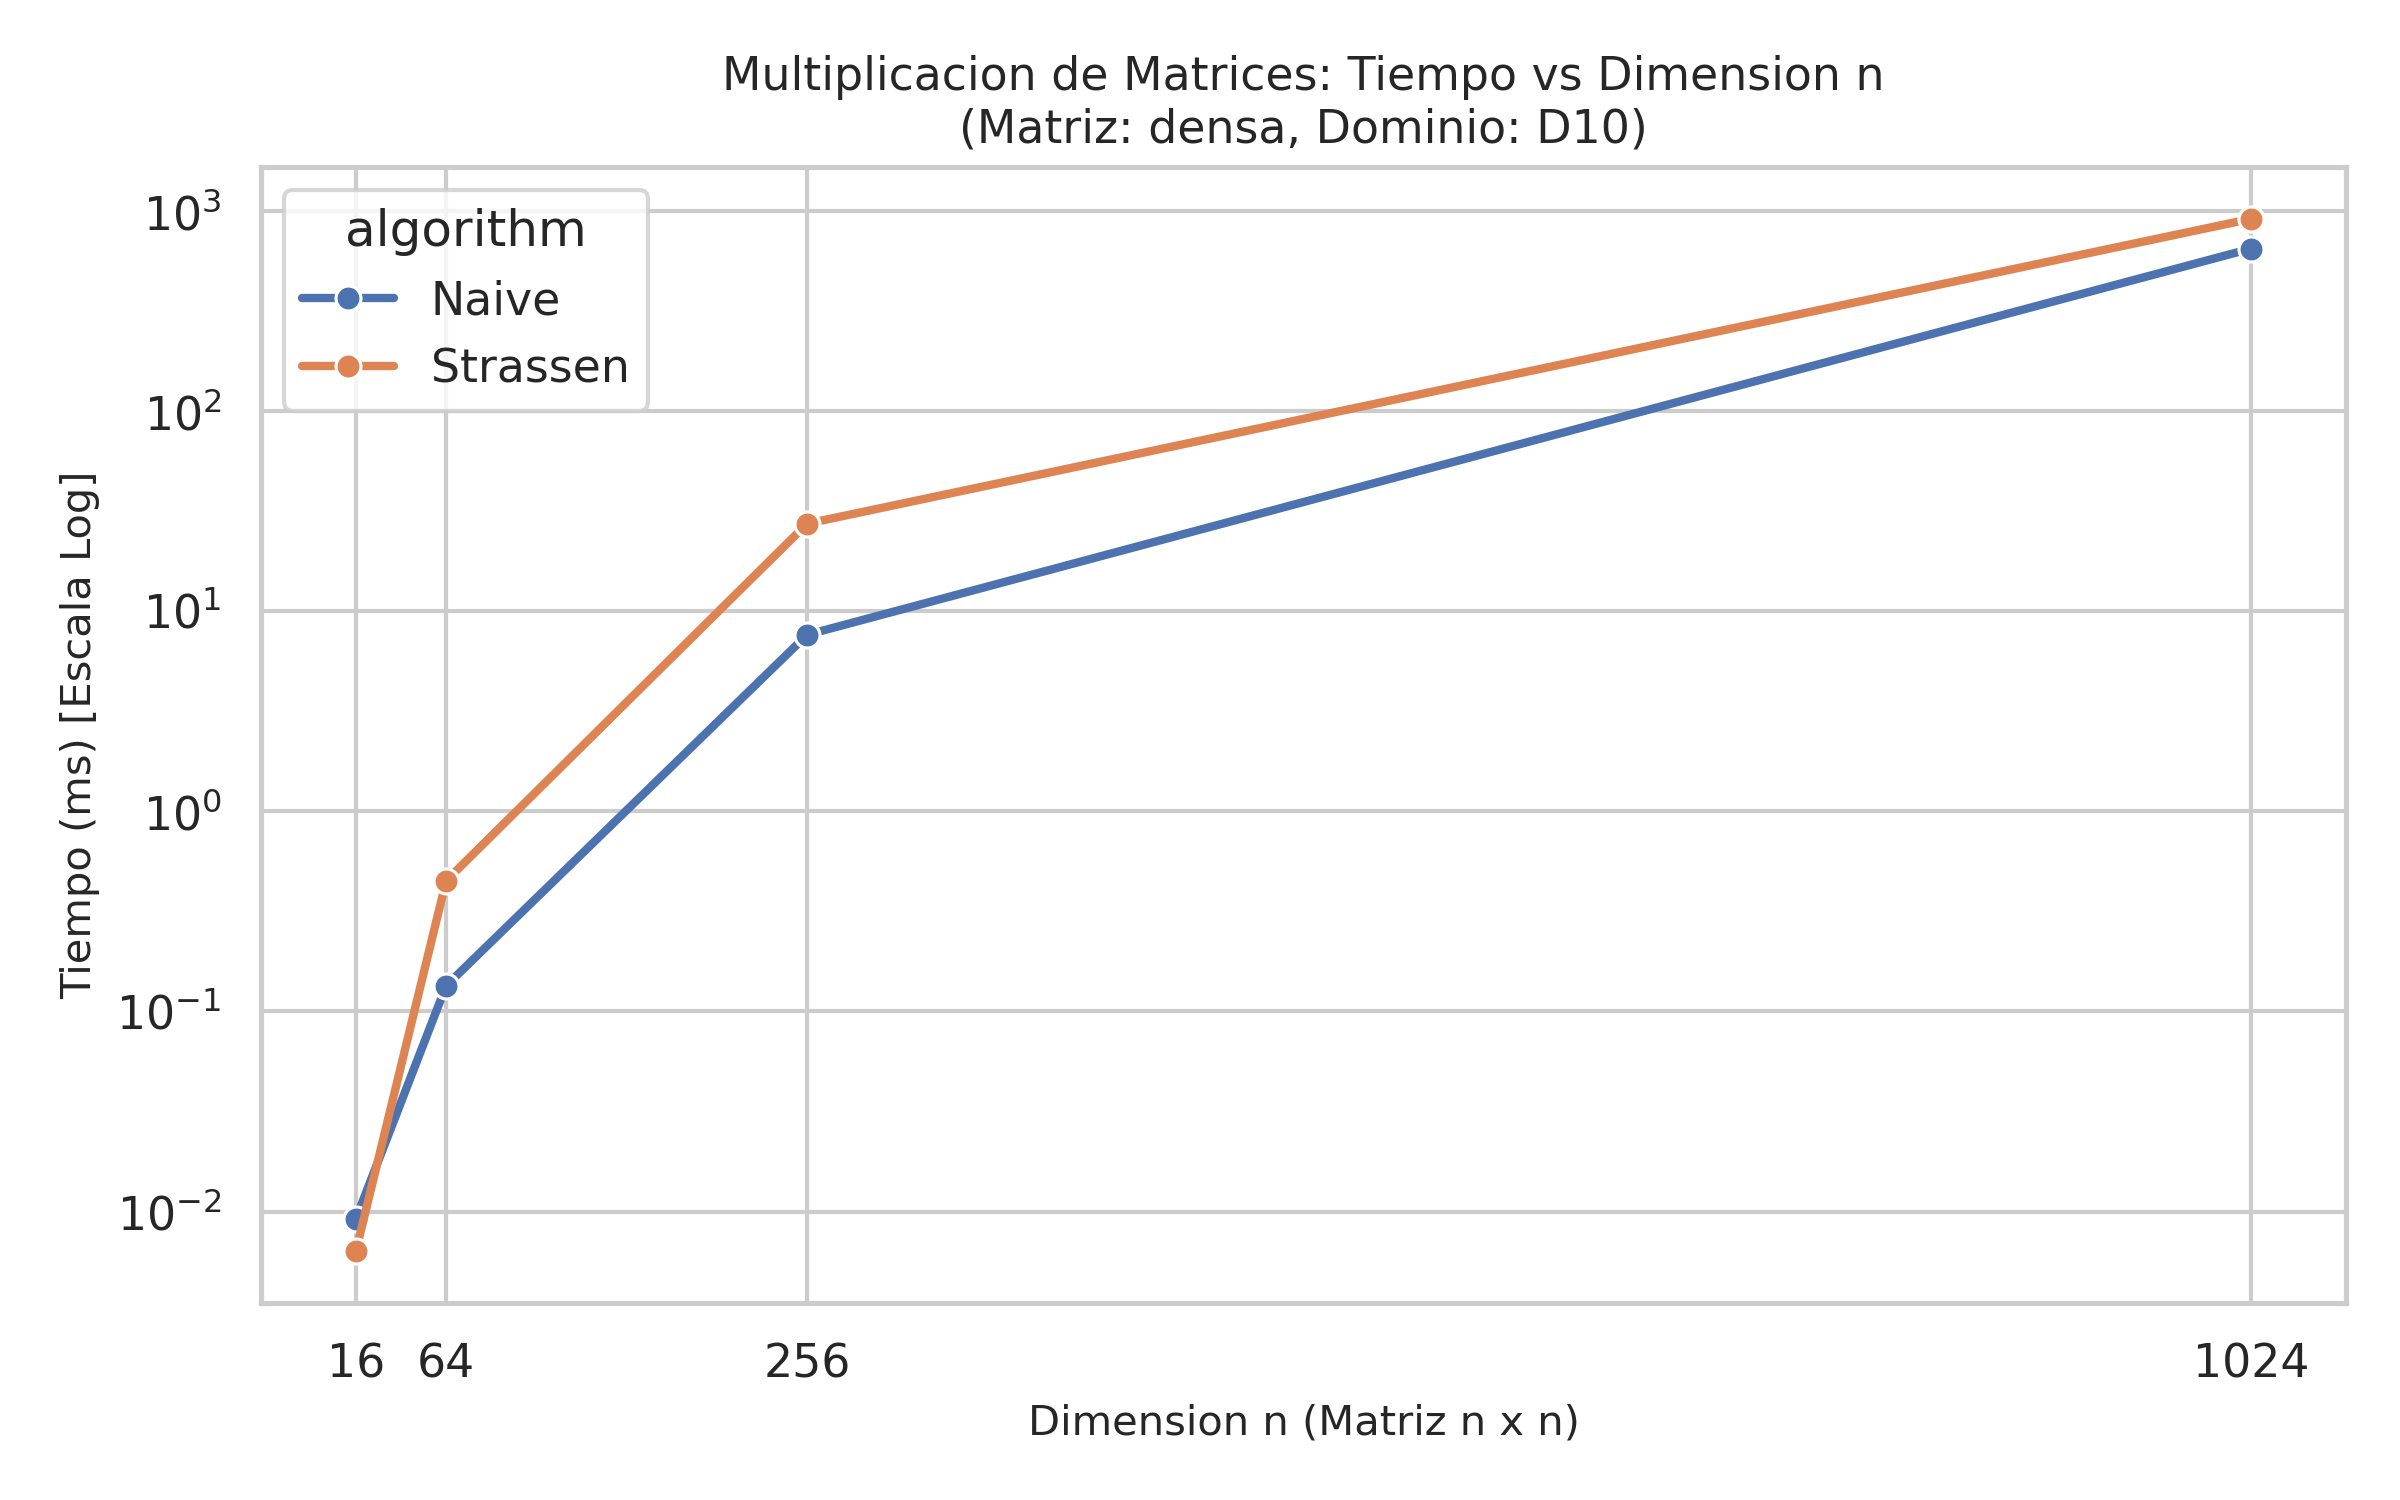
\includegraphics[width=0.85\textwidth]{../code/matrix_multiplication/data/plots/matrix_time_densa_D10.png}
    \caption{Tiempo de ejecución vs. dimensión $n$ para matrices densas en dominio D10.}
    \label{fig:matrix_time}
\end{figure}

A pesar de que teóricamente Strassen tiene una menor complejidad 
asintótica $O(n^{2.81})$ frente a la multiplicación realizada por Naive
con complejidad asintotica $O(n^3)$, Strassen tiene un mayor tiempo de 
ejecución que Naive, esto se debe a que este primer algoritmo 
requiere guardar submatrices intermedias que participan en
un proceso de suma y resta de matrices que busca reducir el numero de llamadas
recursivas, lo que termina provocando un overhead de tiempo de ejecución para
matrices que no son lo suficientemente grandes.

\vspace{0.4cm}

\subsubsection{Consumo de Memoria}

Respecto al consumo de memoria (Peak RSS) utilizado por los algoritmos,
se observa que el algoritmo de Strassen escala de forma drástica al
aumentar la dimensión, alcanzando aproximadamente 6800 KB para $n = 1024$,
mientras que el método Naive se mantiene cercano a 1300 KB, creciendo de
forma lineal, como se muestra en la Figura~\ref{fig:matrix_memory}:

\begin{figure}[H]
    \centering
    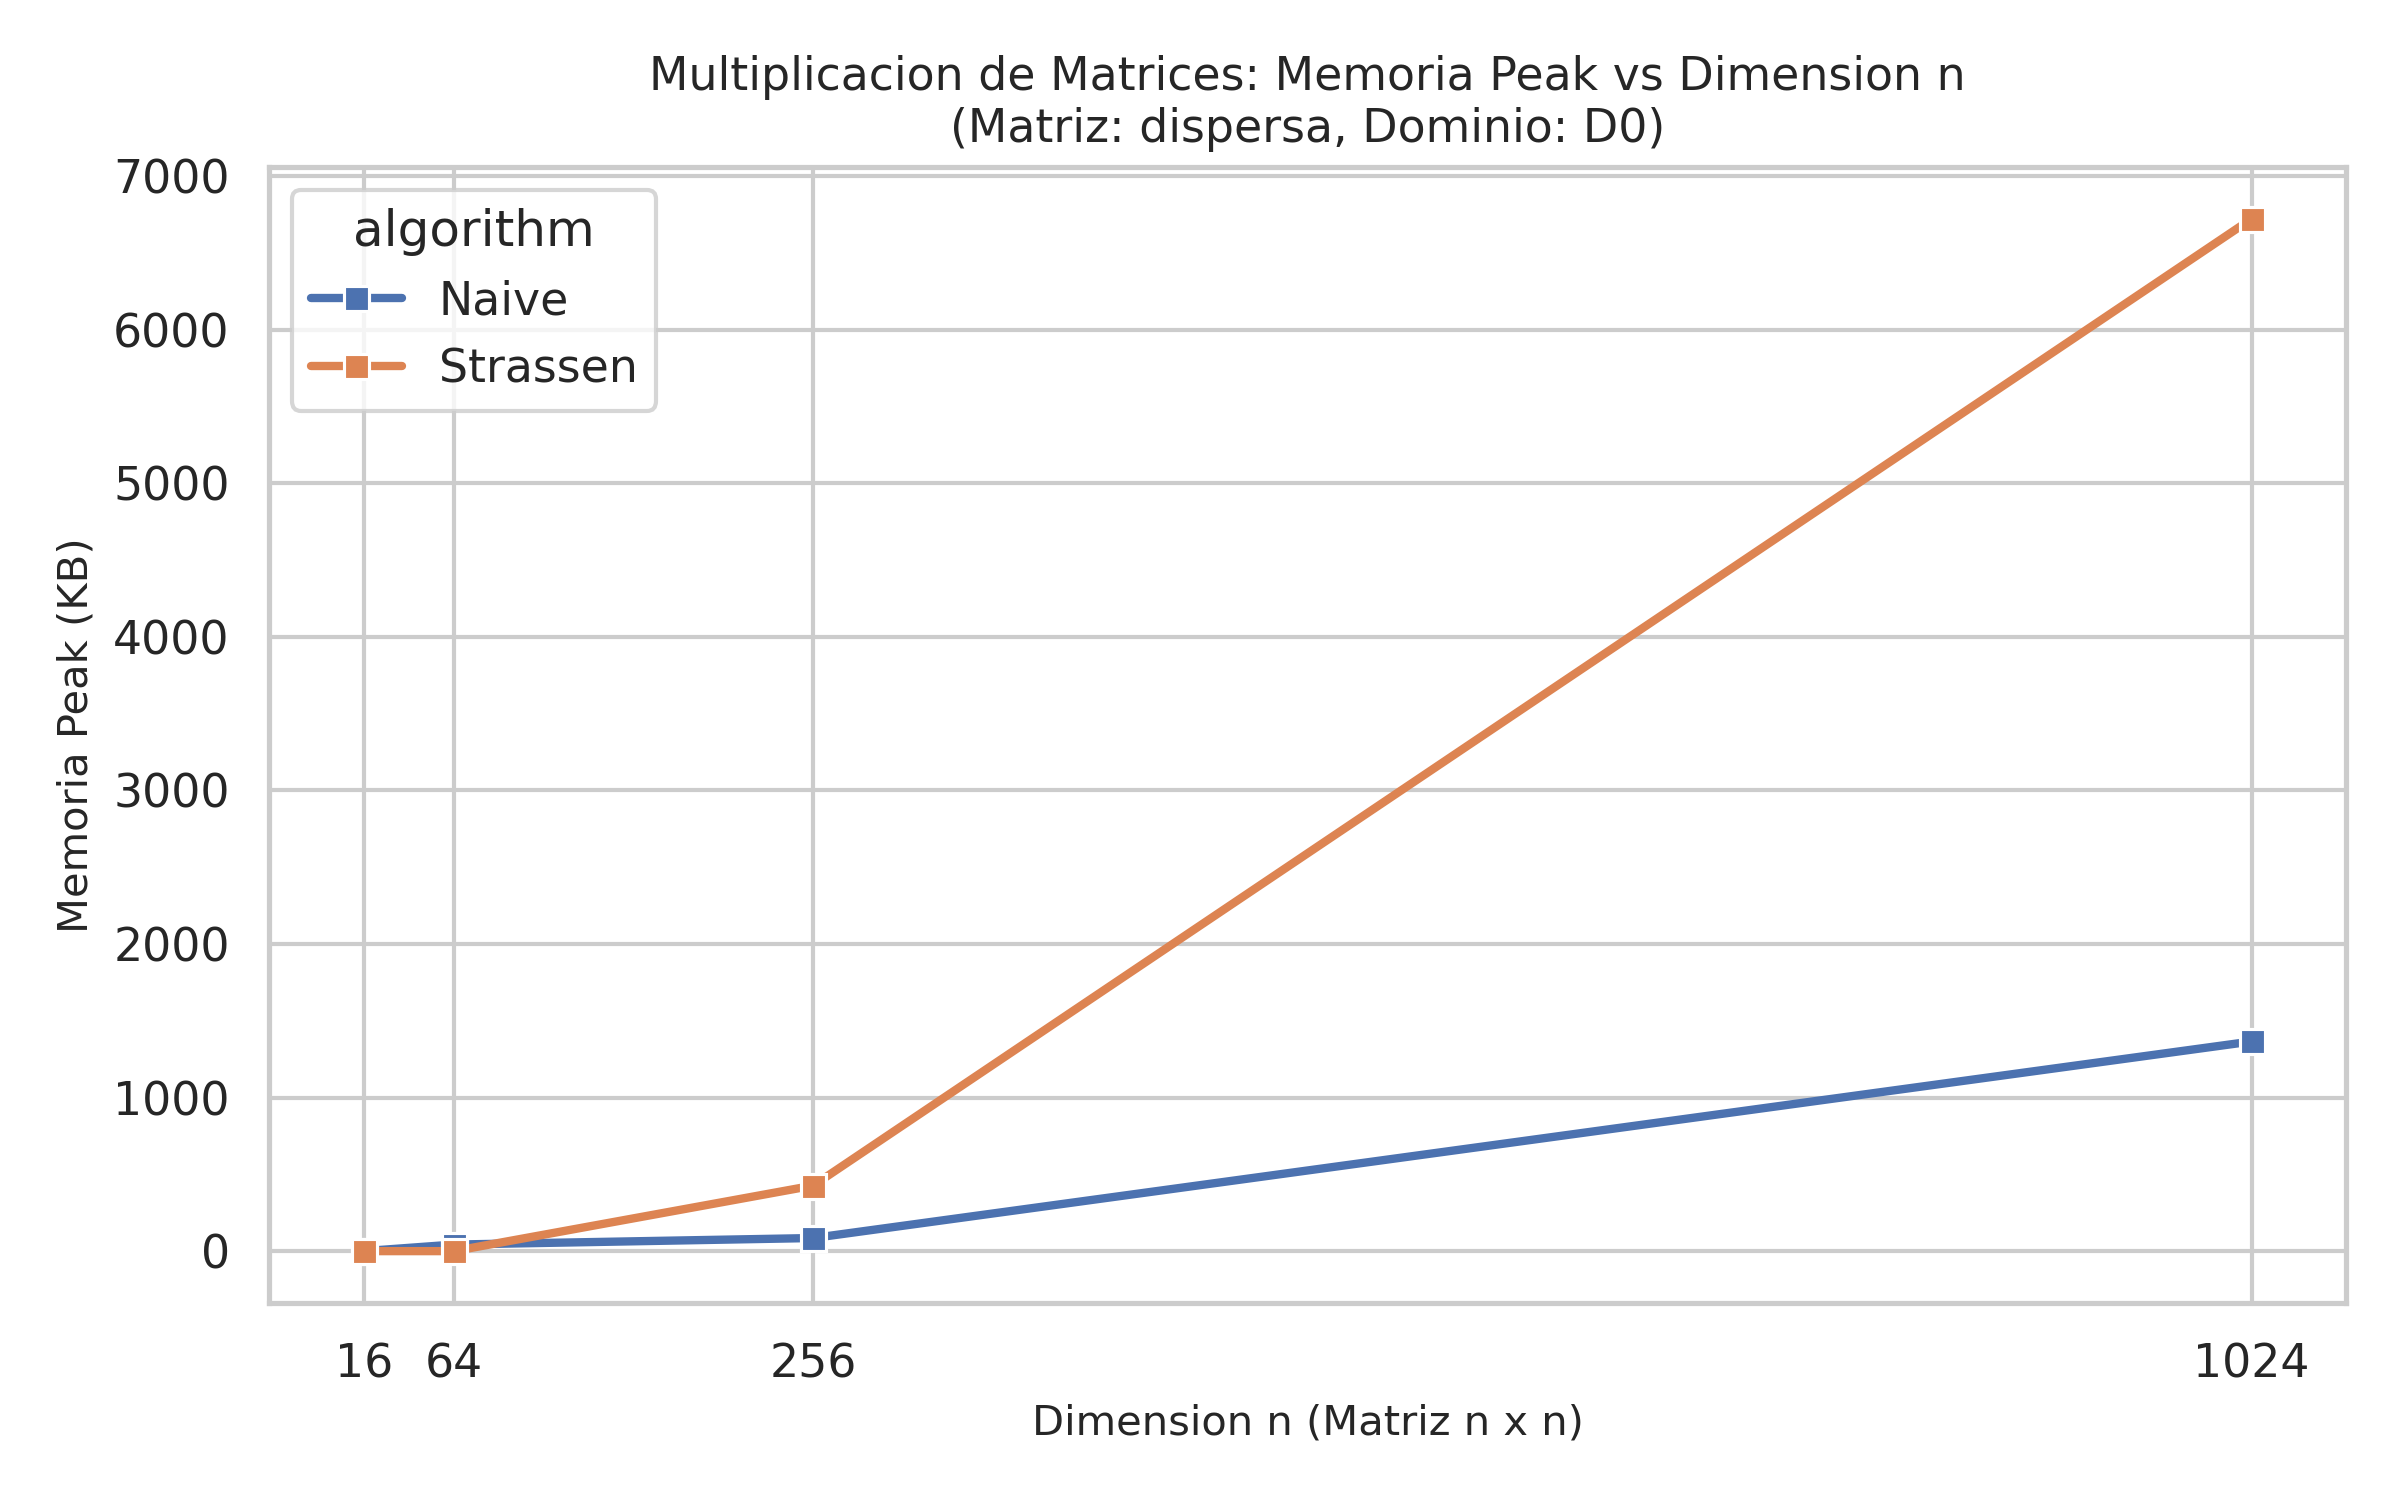
\includegraphics[width=0.85\textwidth]{../code/matrix_multiplication/data/plots/matrix_memory_dispersa_D0.png}
    \caption{Uso de memoria Peak RSS vs. dimensión $n$ para matrices dispersas en dominio D0.}
    \label{fig:matrix_memory}
\end{figure}

Este comportamiento se debe a la creación de 10 submatrices
intermedias ($M_1 \dots M_7$, $A_{11}$, etc.) por cada nivel
de la pila recursiva en el algoritmo de Strassen, resultando en 
un impacto de memoria con un factor constante elevado en comparación
a la estructura estática del método iterativo que utiliza Naive.

\subsection{Ordenamiento de Arreglos Unidimensionales}

\subsubsection{Tiempo de Ejecución}

En el análisis de los resultados experimentales, se observa que los
algoritmos de ordenamiento Quick Sort y Merge Sort presentan un tiempo de ejecución
superior al de los algoritmos Patience Sort y Sort para arreglos ordenados de 
manera descendente, especialmente el algoritmo Quick Sort, del cual no
se tomaron datos para arreglos de tamaño $n = 10^7$, debido al desbordamiento de pila (\textit{Stack Overflow}) y un error de segmentación
(\textit{Segmentation Fault}) al superar el límite del \textit{call stack} del sistema
operativo ($8\,\text{MB}$)..

\vspace{0.4cm}

El algoritmos Sort fue el de mejor desempeño en cuanto a tiempo de ejecución,
mientras que Patience Sort y Merge Sort mostraron un desempeño comparable 
a la par de estabilidad en todas las configuraciones, manteniendo una curva
asintótica parecida a $O(n \log n)$, como se aprecia en la Figura~\ref{fig:sorting_time}:

\begin{figure}[H]
    \centering
    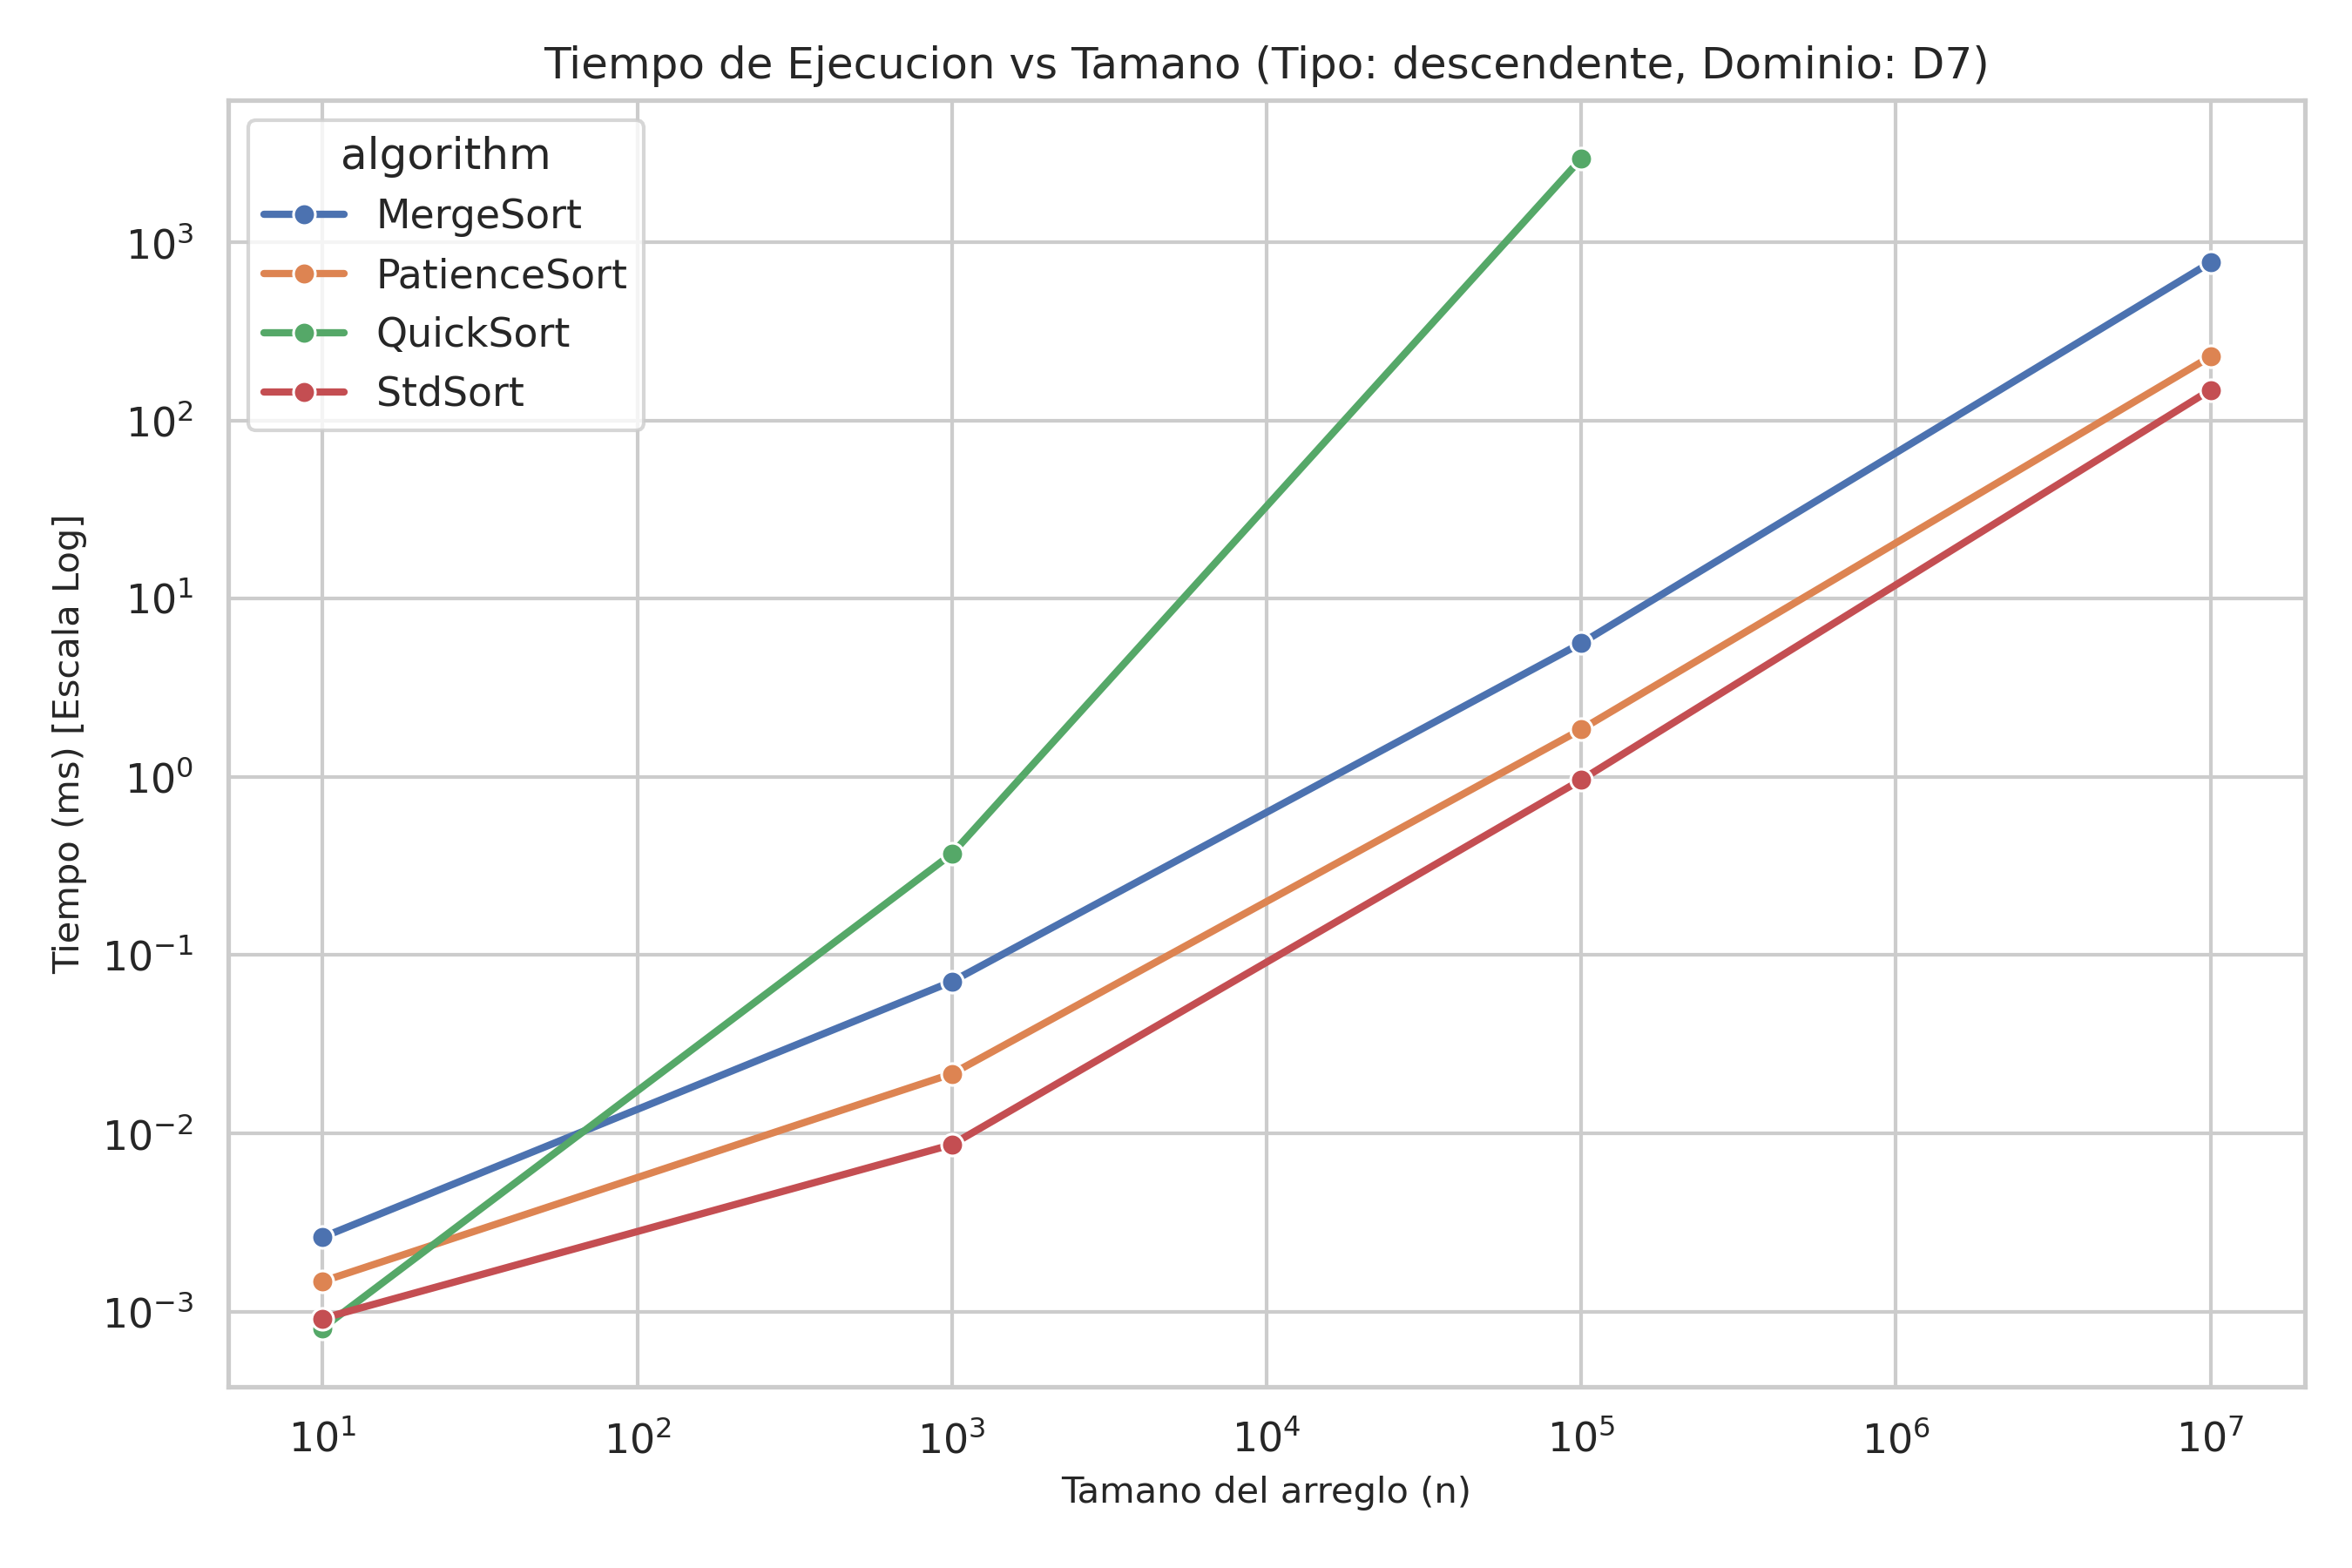
\includegraphics[width=0.85\textwidth]{../code/sorting/data/plots/time_descendente_D7.png}
    \caption{Tiempo de ejecución vs. tamaño $n$ para arreglo descendente en dominio D7.}
    \label{fig:sorting_time}
\end{figure}

El comportamiento observado en los algoritmos de ordenamiento coincide 
con la complejidad asintótica teórica de cada uno, donde Quick Sort, con
$O(n^2)$ cae en el peor caso por tratarse de un arreglo ordenado, causando
una recursion completamente desbalanceada, mientras 
que Patience Sort, que también cuenta con tiempo $O(n^2)$ presenta un tiempo
promedio bastante estable parecido a $O(n \log n)$, el cual incluso supera en la practica al
algoritmo Merge Sort, con tiempo estable $\Theta(n \log n)$, ambos tienen una curva 
muy similar al algoritmo Sort, que también tiene un tiempo promedio de $\Theta(n \log n)$
y un comportamiento estable en todos los rangos de $n$ evaluados.

\vspace{0.4cm}

Este último algoritmo logra su eficiencia gracias a su naturaleza híbrida IntroSorty 
optimizaciones a nivel de compilador, logrando los menores tiempos de ejecución en
comparación a los otros algoritmos con complejidad asintotica similar.

\subsubsection{Consumo de Memoria}

Respecto al consumo de memoria (Peak RSS) utilizado por los algoritmos, se observa que
el algoritmo de Merge Sort escala de forma drástica al aumentar el tamaño del
arreglo, alcanzando aproximadamente 12000 KB para $n = 10^7$, mientras que el método
Sort se mantiene cercano a 1800 KB, creciendo de forma lineal.

\vspace{0.4cm}

Por otro lado, los algoritmos Sort y Quick Sort muestran un comportamiento
imperceptible de uso de memoria, permaneciendo sobre la linea de 0 KB,
como se muestra en la Figura~\ref{fig:sorting_memory}:

\begin{figure}[H]
    \centering
    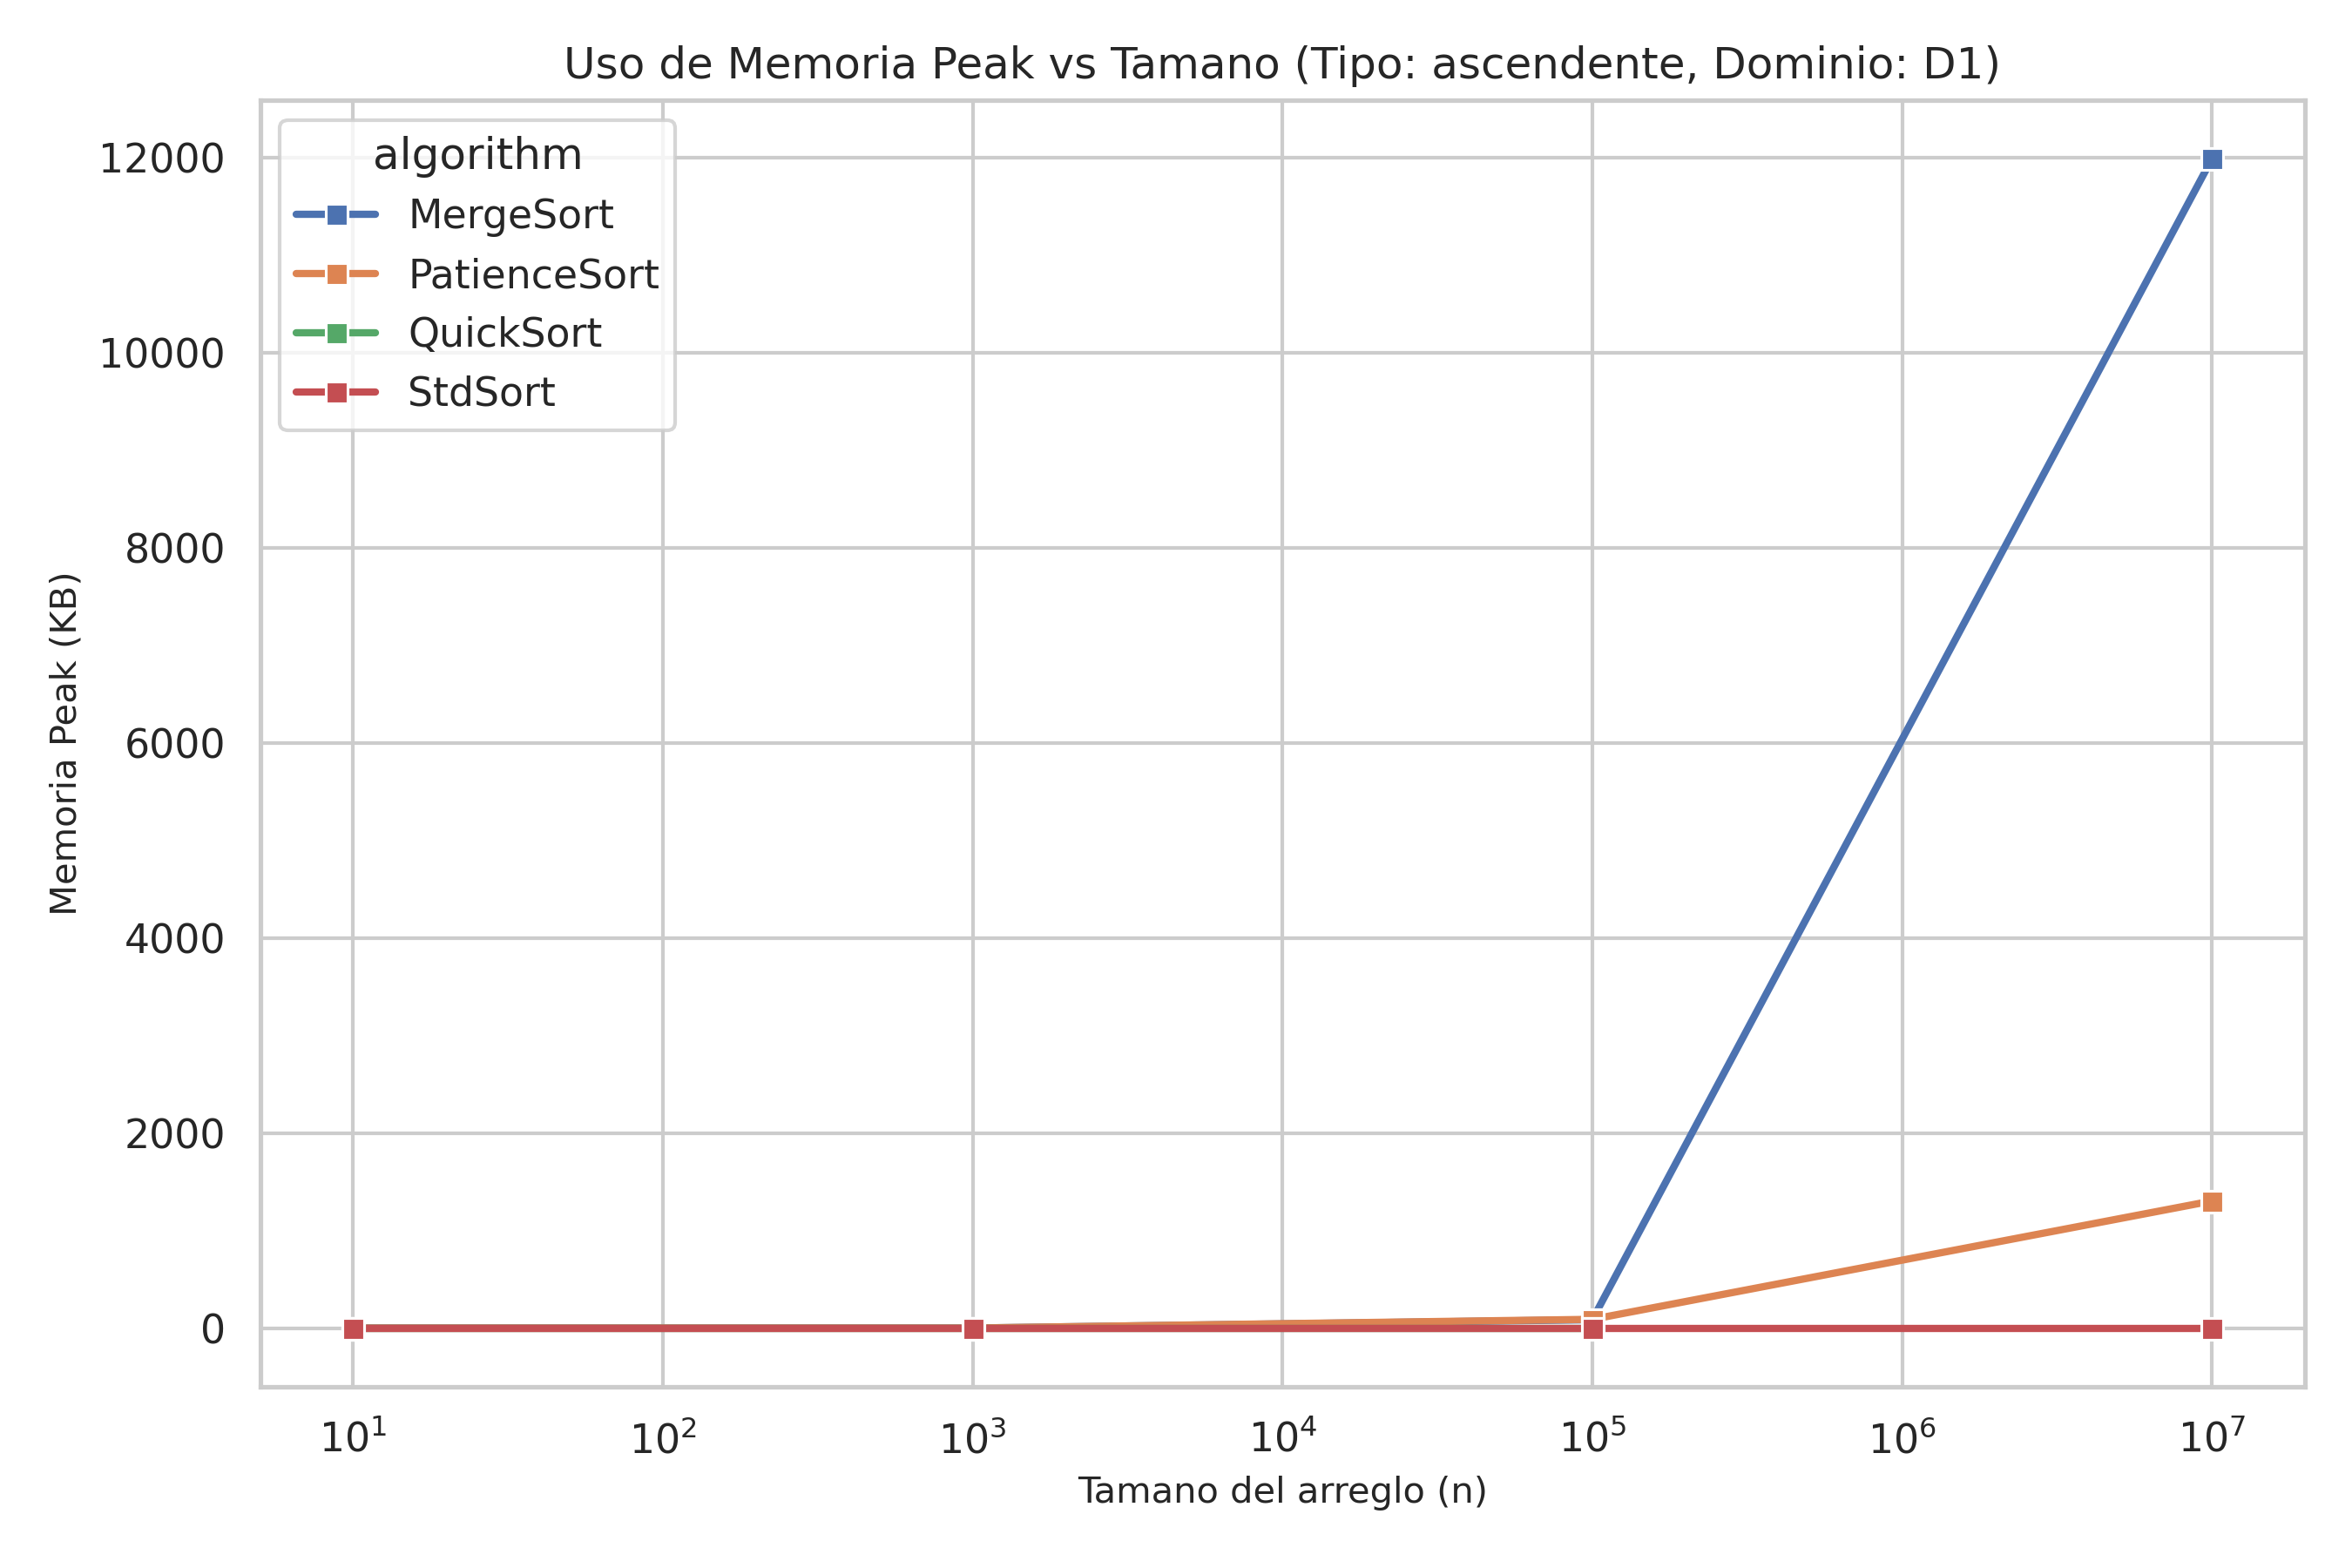
\includegraphics[width=0.85\textwidth]{../code/sorting/data/plots/memory_ascendente_D1.png}
    \caption{Uso de memoria Peak RSS vs. tamaño $n$ para arreglo ascendente en dominio D1.}
    \label{fig:sorting_memory}
\end{figure}

El comportamiento observado en los algoritmos de ordenamiento coincide con la
complejidad asintótica teórica de cada uno, donde Merge Sort exhibe una asignación
auxiliar proporcional a $O(n)$ debido a los vectores temporales en la fase de fusión,
mientras que Sort mantiene un uso de memoria mínimo, con $O(1)$ en el consumo de memoria, 
realizando el ordenamiento in-place sin requerir espacio adicional significativo.

\vspace{0.4cm}

En el caso de Quick Sort y Sort, ambos son algoritmos in-place. 
La única memoria adicional consumida proviene del marco de llamadas
de la pila de recursión, lo cual es prácticamente imperceptible a
nivel del sistema operativo en términos de Peak RSS.